%%%%%%%%%%%%%%%%%%%%%%%%%%%%%%%%%%%%%%%%%%%%%%%%%%%%%%%%%%%%%%%%
%      材料学会投稿用TeXサンプルファイル  Ver2.0
%      作成日:2019年9月22日
%      作成者:Aoi Watanabe
%%%%%%%%%%%%%%%%%%%%%%%%%%%%%%%%%%%%%%%%%%%%%%%%%%%%%%%%%%%%%%%%
\documentclass{ujarticle}
%
\usepackage{jsms2019}% 材料スタイルファイル
\usepackage{epic,eepic}% Fig関係
\usepackage[dvips]{graphicx}% \includegraphics
\usepackage{here}% 図表の位置を強制指定(位置指定にHを使用)
\usepackage{color}% 著者情報の白点の入力に必要
\usepackage{amsmath}% 数式,boldsymbolの利用など(ams*** は米国数学会のスタイル)
\usepackage{amssymb}
%
\renewcommand{\rmdefault}{ptm}% 標準のフォントをTimesに変更
%
%\bibliographystyle{jplain}
%
%%%%%%%%%%%%%%%%%%%%%%%%%%%%%%%%%%%%%%%%%%%%%%%%%%%%%%%%%%%%%
%   マクロ定義はここで宣言しておく
%%%%%%%%%%%%%%%%%%%%%%%%%%%%%%%%%%%%%%%%%%%%%%%%%%%%%%%%%%%%%
\def\HLINE{\noalign{\hrule height1pt}}    % 表で使う太線
\def\degC{\kern-.2em\r{}\kern-.3em C}   % ℃の出力
%
%----- 式番号の右を少し開ける数式の環境 -----
\newenvironment{jsmseq}
{
\vspace*{-1mm}
\begin{flushleft}
\begin{minipage}{0.45\textwidth}
\begin{equation}
}
{
\end{equation}
%\vskip 1mm
\end{minipage}
\end{flushleft}
}
%
%%%%%%%%%%%%%%%%%%%%%%%%%%%%%%%%%%%%%%%%%%%%%%%%%%%%%%%%%%%%%
%   文書の開始
%%%%%%%%%%%%%%%%%%%%%%%%%%%%%%%%%%%%%%%%%%%%%%%%%%%%%%%%%%%%%
\begin{document}
\unitlength 1mm
%
%%%%%%%%%%%%%%%%%%%%%%%%%%%%%%%%%%%%%%%%%%%%%%%%%%%%%%%%%%%%%
%   和文タイトルの記述
%   (1)\fontsize{15pt}{20pt}は,フォントの大きさを15ポイント,
%      行送りを20ポイントに指定することを意味する
%      行送りについては適宜調整する必要あり
%   (2)コンパイル後にフォントがない旨のメッセージが出るが
%      確認した限り指定した大きさに調整はされている
%%%%%%%%%%%%%%%%%%%%%%%%%%%%%%%%%%%%%%%%%%%%%%%%%%%%%%%%%%%%%
\begin{center}
{\fontsize{15pt}{20pt}\selectfont   % Times 15pt
和文タイトル:材料学会\LaTeX テンプレートVer 1.1 ${^\dag}$\\
}
\end{center}

%%%%%%%%%%%%%%%%%%%%%%%%%%%%%%%%%%%%%%%%%%%%%%%%%%%%%%%%%%%%%
%   和文著者の記述
%   著者間の
%   \hspace*{-1zw}\textcolor{white}{\textbullet}
%   は,白点を出力するのに使っている.印刷所で必要になるので必ず入れて下さい.
%%%%%%%%%%%%%%%%%%%%%%%%%%%%%%%%%%%%%%%%%%%%%%%%%%%%%%%%%%%%%
\begin{flushright}
{\fontsize{11pt}{0pt}\selectfont    % Times 11pt
%\large
\begin{tabular}{lll}
%%%
材料\hspace{1zw}一郎 $^{\ast}$
%%%
&
\hspace*{-1zw}\textcolor{white}{\textbullet} % white dot
%%%
材料\hspace{1zw}次郎 $^{\ast\ast}$
%%%
&
\hspace*{-1zw}\textcolor{white}{\textbullet} % white dot
%%%
材料\hspace{1zw}三郎 $^{\ast}$
%%%
\\[2mm]%
%\hspace*{-1zw}\textcolor{white}{\textbullet} % white dot
%%%
%材料\hspace{1zw}三四郎$^{\ast\ast}$
%%%
&
\hspace*{-1zw}\textcolor{white}{\textbullet} % white dot
%%%
材料\hspace{1zw}四郎$^{\ast\ast}$
%%%
&
\hspace*{-1zw}\textcolor{white}{\textbullet} % white dot
%%%
材料\hspace{1zw}五郎$^{\ast\ast\ast}$
%%%
 \end{tabular}
 }
\end{flushright}

\vspace*{-2mm}  %   縦方向の隙間の調整(必要箇所に適宜挿入)
%%%%%%%%%%%%%%%%%%%%%%%%%%%%%%%%%%%%%%%%%%%%%%%%%%%%%%%%%%%%%
%   英文タイトルの記述
%   2行に渡る場合はフォントサイズ指定の行送りで行間を調整する
%%%%%%%%%%%%%%%%%%%%%%%%%%%%%%%%%%%%%%%%%%%%%%%%%%%%%%%%%%%%%
\begin{center}
{\fontsize{13pt}{0pt}\selectfont  % Times 13 pt
A Sample of Manuscript of Submitted Paper to
\\[1mm]
Journal of the Society of Materials Science, Japan
}
\end{center}

\vspace*{-4mm}   %   縦方向の隙間の調整
\begin{center}
{\small by}
\end{center}

\vspace*{-2mm}   %   縦方向の隙間の調整
%%%%%%%%%%%%%%%%%%%%%%%%%%%%%%%%%%%%%%%%%%%%%%%%%%%%%%%%%%%%%
%   英文著者の記述
%   2行に渡る場合はフォントサイズ指定の行送りで行間を調整する
%%%%%%%%%%%%%%%%%%%%%%%%%%%%%%%%%%%%%%%%%%%%%%%%%%%%%%%%%%%%%
\begin{center}
 {\fontsize{10.5pt}{0pt}\selectfont  % Times 10.5ps
%%%
Ichiro\ Z{\fontsize{7pt}{0pt}\selectfont AIRYO}$^{\ast}$, 
%%%
Jiro\ Z{\fontsize{7pt}{0pt}\selectfont AIRYO}$^{\ast\ast}$, 
%%%
Saburo\ Z{\fontsize{7pt}{0pt}\selectfont AIRYO}$^{\ast\ast}$, 
%%%
\\
%%%
Shiro\ Z{\fontsize{7pt}{0pt}\selectfont AIRYO}$^{\ast\ast}$, 
%%%
Goro\ Z{\fontsize{7pt}{0pt}\selectfont AIRYO}$^{\ast\ast\ast}$
%%%
}
\end{center}


\vspace*{0mm}   %   縦方向の隙間の調整
%%%%%%%%%%%%%%%%%%%%%%%%%%%%%%%%%%%%%%%%%%%%%%%%%%%%%%%%%%%%%
%   英文アブストラクトの記述
%%%%%%%%%%%%%%%%%%%%%%%%%%%%%%%%%%%%%%%%%%%%%%%%%%%%%%%%%%%%%
\begin{center}
\begin{minipage}{160mm}
\baselineskip 12pt%minipage内の行間のローカルな調整
\setlength{\parindent}{4mm} %minipage内のインデントのローカルな調整
{\fontsize{9.5pt}{0pt}\selectfont   % Times 9.5 pt
%%%%% アブストラクト記入はじまり %%%%%
Wide-bandgap semiconductor ZnO potentially exhibits high radiation hardness since large displacement threshold energy of constituent atoms can be expected due to the small lattice constant and large bandgap energy. To study the radiation hardness, the effect of proton irradiation on single-crystalline $n$-type ZnO films was examined. These films were grown by molecular beam epitaxy, and irradiated by $8$~MeV protons with fluences of
$1.4\times 10^{15}$, $2.8\times 10^{15}$, $5.6\times 10^{15}$ and $1.4\times 10^{16}$~p/cm$^2$. A rapid increase of electrical resistance by a decrease of carrier density was observed with a threshold fluence of about $1\times 10^{15}$~p/cm$^2$. This change in electrical properties was associated with a steep deterioration of the near-bandedge emission intensity in cathodoluminescence. These radiation damages were found to recover after a thermal annealing over $600$\degC. Such high radiation hardness of ZnO exceeds that of GaN, indicating promising application of this material to space- and nuclear-electronics. 
%%%%% アブストラクト記入おわり %%%%%%
}
\end{minipage}
\end{center}

%%%%%%%%%%%%%%%%%%%%%%%%%%%%%%%%%%%%%%%%%%%%%%%%%%%%%%%%%%%%%
%   英文キーワードの記述
%%%%%%%%%%%%%%%%%%%%%%%%%%%%%%%%%%%%%%%%%%%%%%%%%%%%%%%%%%%%%
\vspace*{-2.5mm}
\hspace*{8mm}{\fontfamily{qbk}\fontsize{9.5pt}{0pt}\selectfont  %Bookman Old Style 9.5 pt
\textbf{\textit{Key words:}}
}

\vspace*{-2.5mm}
\begin{center}
\begin{minipage}{130mm}
\baselineskip 12pt
{\fontfamily{pnc}\fontsize{9.5pt}{0pt}\selectfont  %New Century Font 9.5 pt
%%%%% 英文キーワード記入はじまり %%%%%
ZnO, 8 MeV protons, Radiation damage, Radiation hardness, 
Thermal annealing, xxx xxx xxxxx, xxxxxxxx, xxx, xxxxxxx xxxx
%%%%% 英文キーワード記入おわり %%%%%%
}
\end{minipage}
\end{center}

%%%%%%%%%%%%%%%%%%%%%%%%%%%%%%%%%%%%%%%%%%%%%%%%%%%%%%%%%%%%%
%     著者の所属などのフッターを記入
%%%%%%%%%%%%%%%%%%%%%%%%%%%%%%%%%%%%%%%%%%%%%%%%%%%%%%%%%%%%%
\def\thefootnote{\fnsymbol{footnote}}
\def\footnotesize{\fontsize{7pt}{0pt}\selectfont}   %Times 7pt
%
\footnotetext[0]{
\baselineskip 9.5pt
\hspace*{-5mm}
%
\parbox[l]{4mm}{$\dag$}
原稿受理 平成  年  月  日 Received  \hspace*{18mm} \copyright  2011 The Society of Materials Science, Japan \\
%%%%%%%%%%%%% Affiliation 1 %%%%%%%%%%%%%%%
% ※Web掲載のフォーマットに従い和文と英文は別の行で書く形式にしている.
%   改行なし(以前の形式)で書いても良いとのこと.著者名が多い場合は誌面の節約になる.
%%%%%%%%%%%%%%%%%%%%%%%%%%%%%%%%%%%%%%
\parbox[l]{4mm}{$\ast$}
正 会 員 京都大学大学院 工学研究科 機械理工学専攻 〒615-8540 京都市西京区京都大学桂\\
%
\parbox[l]{4mm}{\textcolor{white}{$\ast$}}    %白色で*を出力(印刷所で必要)
 {\fontfamily{pnc} \selectfont  % New Century Font 7 pt 
Department of Mechanical Engineering and Science, Graduate School of Engineering, Kyoto University, Kyoto-Daigaku-Katsura, Nishikyo-ku,} \linebreak 
\parbox[l]{4mm}{\ }
 {\fontfamily{pnc} \selectfont  % New Century Font 7 pt 
Kyoto 615-8540.} \\
%%%%%%%%%%%%%%%%%%%%%%%%%%%%%%%%%%%%%%
%%%%%%%%%%%%% Affiliation 2 %%%%%%%%%%%%%%%
\parbox[l]{4mm}{$\ast\hspace*{-0.5mm}\ast$}
九州工業大学大学院 情報工学研究科 情報システム専攻 〒820-8502 福岡県飯塚市川津\\
%
\parbox[l]{4mm}{\textcolor{white}{$\ast\hspace*{-0.5mm}\ast$}}  %白色で*を出力(印刷所で必要)
{\fontfamily{pnc} \selectfont  % New Century Font 7 pt 
Graduate School of Computer Science and Systems Engineering, Kyushu Institute of Technology, Kawazu, Iizuka, Fukuoka 820-8502.}\\
%%%%%%%%%%%%%%%%%%%%%%%%%%%%%%%%%%%%%%
%%%%%%%%%%%%% Affiliation 3 %%%%%%%%%%%%%%%
\parbox[l]{4mm}{$\ast\hspace*{-0.5mm}\ast\hspace*{-0.5mm}\ast$}
大阪大学大学院 工学研究科 知能・機能創成工学専攻 〒565-0871 大阪府吹田市山田丘2番1号\\
\parbox[l]{4mm}{\textcolor{white}{$\ast\hspace*{-0.5mm}\ast\hspace*{-0.5mm}\ast$}}  %白色で*を出力(印刷所で必要)
{\fontfamily{pnc} \selectfont  % New Century Font 7 pt 
Department of Adaptive Machine Systems, Graduate School of Engineering, Osaka University, 2-1 Yamadaoka, Suita, Osaka 565-0871.}
%%%%%%%%%%%%%%%%%%%%%%%%%%%%%%%%%%%%%%
}

%%%%%%%%%%%%%%%%%%%%%%%%%%%%%%%%%%%%%%%%%%%%%%%%%%%%%%%%%%%%%
%   メインテキストの開始位置,文字サイズなどの設定
%%%%%%%%%%%%%%%%%%%%%%%%%%%%%%%%%%%%%%%%%%%%%%%%%%%%%%%%%%%%%
\vspace*{-2mm}
{\small  % 本文中のフォントを9ptに変更
\begin{multicols}{2}
\baselineskip 14.1pt
%%%%%%%%%%%%%%%%%%%%%%%%%%%%%%%%%%%%%%%%%%%%%%%%%%%%%%%%%%%%%
%   本文の入力の開始
%%%%%%%%%%%%%%%%%%%%%%%%%%%%%%%%%%%%%%%%%%%%%%%%%%%%%%%%%%%%%
\section{緒\hspace{4zw}言}

日本材料学会会誌「材料」に投稿できる原稿は,投稿規定6.に定める論文,資料,総説,講座,解説,国内外トピックス,
委員会報告,巻頭言,討論,会員便りのいずれかである.

論文はその内容が一般に公表されている国内外の印刷物に未投稿のものであって,理論,実験等に誤りがなく,
材料学に関して独創的な研究で,価値ある結論あるいは事実を含むものでなければならない.

それぞれの原稿は,A4用紙に25字×51行×2段=2550字,横書き(刷上がり1ページに相当)に執筆する.
所定の投稿申込用紙と,「投稿原稿見本」に従って作成した投稿原稿のPDFファイルを本会編集委員会宛に提出する.
正原稿は編集委員会において掲載可が決定され本会より提出の依頼があるまで著者が保管する.

\subsection{原稿の執筆上の注意}

原稿の書き方は,投稿規程および原稿執筆上の規約に従う必要があるが,第1ページおよび図などは本ページに示す見本を参照するとよい.
左右に21mm,上23mm,下18mmのマージンをとる.本文は2段組としコラム幅は80mm,コラム間隔を10mmとする.
論文および資料の場合,次の事項を番号順に必ず記載する.(1)和文題名(15ポイント),(2)和文著者名(11ポイント),
(3)英文題名(13ポイント),(4)英文著者名(10.5ポイント),(5)英文要旨(9.5ポイント),(6)英文キーワード(9.5ポイント).
また,最下段に本文との間に線を入れて(7)和文の会員種別・所属・所在地,英文の所属・所在地を記載する.
その他の原稿では記載事項が異なるので原稿執筆上の規約を参照すること.

本文(9ポイント)は,見本のように上記(1)~(6)を記述した後に,1行空けて書き始める.

図,表および写真は,論文,資料,委員会報告については,見本のように用紙にそのまま貼り込める大きさに用意し,
本文中の説明と離れない位置に貼り付ける.図・表どうし,あるいは図,表と本文は1行以上間隔をあけるようにする.
カラー写真掲載希望の場合は,編集委員会でその必要性が認められた場合に限り掲載することができるが,
それに係わる経費は著者負担である.
\newpage
\section{ABC照射試料の準備}

分子線エピタキシー(MBE)装置を用いてFig. 1に示すノンドープの単結晶ZnO薄膜を作製した.
まず,A面サファイア基板上に15~nmのZn$_{0.85}$Mg$_{0.15}$O薄膜を300\degC で成膜した.
真空中で800\degC ・30分間の熱処理を経て,300

%%%% Equation 1 %%%%%%%%%%%%%%%%%%%%%
% 冒頭で定義したjsmseq環境を使用
%       (材料のフォーマットに合わせて式番号の右にスペースが入る)
\begin{jsmseq}
	\frac{\mathrm{d}\sigma}{\mathrm{d}\Omega}
	=
	\left(
		\frac{Z_{1}Z_{2}e^{2}}{8\pi\varepsilon_{0}M_{1}\nu^{2}}
	\right)^{2}
	\mathrm{cosec}^{4}\frac{\theta}{2}
\label{eq:1}   % 式のラベル
\end{jsmseq}
%%%%%%%%%%%%%%%%%%%%%%%%%%%%%%%%%%

%%%%% Fig.1 (二段組中の図)%%%%%%%%
\begin{figure}[H]
	\centering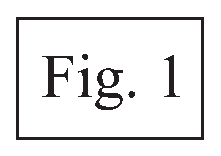
\includegraphics[keepaspectratio, width=50mm]{images/Fig1.eps} %[図のサイズ指定]{ファイル名}
	\caption{Schematic diagram of a sample structure.} % 表題
	\label{fig1}  % ラベル
\end{figure}
%%%%%%%%%%%%%%%%%%%%%%%%%%%%%%%

%%%%% Table 1 (二段組中の表)%%%%%%
\begin{table}[H]
	\caption{Electrical properties of a single-crystalline ZnO film.}
	\label{table1}
	\begin{center}
		\small
		\begin{tabular}{cccc}
			\HLINE
			& Resistivity & Hall mobility & Carrier density \\ 
			& ($\Omega$) & (cm$^2$/Vs) & (cm$^{-3}$)  \\ 
			\HLINE
			300~K & 0.107 & 103 & 5.64$\times$10$^{-17}$ \\ 
			700~K & 0.273 & 302 & 7.57$\times$10$^{-16}$ \\ 
			\HLINE
		\end{tabular}
	\end{center}
\end{table}
%%%%%%%%%%%%%%%%%%%%%%%%%%%%%%%%

%%%%%% Table 2 (一段組み)%%%%%%%%%%
%\begin{table*}[tb]
%	\caption{Electrical properties of a single-crystalline ZnO film.}
%	\label{table2}
%	\begin{center}
%		\small
%		\begin{tabular}{cccc}
%			\HLINE
%			& Resistivity & Hall mobility & Carrier density \\ 
%			& ($\Omega$) & (cm$^2$/Vs) & (cm$^{-3}$)  \\ 
%			\HLINE
%			300~K & 0.107 & 103 & 5.64$\times$10$^{-17}$ \\ 
%			700~K & 0.273 & 302 & 7.57$\times$10$^{-16}$ \\ 
%			\HLINE
%		\end{tabular}
%	\end{center}
%\end{table*}
%%%%%%%%%%%%%%%%%%%%%%%%%%%%%%%%

%%%%%% Fig. 2(図を並べて配置)%%%%%%%
\begin{figure}[H]
	\begin{center}
		\begin{minipage}{35mm}
			\centering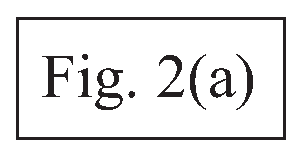
\includegraphics[keepaspectratio, width=30mm]{images/Fig2a.eps}\\
			\fontsize{8.5pt}{0pt}\selectfont{(a) Left figure}
		\end{minipage}
		\hspace{5mm}
		\begin{minipage}{35mm}
			\centering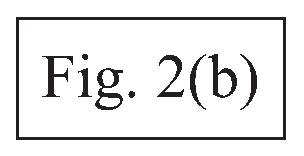
\includegraphics[keepaspectratio, width=30mm]{images/Fig2b.eps}\\
			\fontsize{8.5pt}{0pt}\selectfont{(b) Right figure}
		\end{minipage}
	\end{center}
	\caption{Schematic diagram of an experimental setup of 8~MeV proton beam irradiation.}
	\label{fig2}
\end{figure}
%%%%%%%%%%%%%%%%%%%%%%%%%%%%%%%%%

%%%%%%%% Fig. 3 (一段組み)%%%%%%%%%%%
\begin{figure*}[t]
	\centering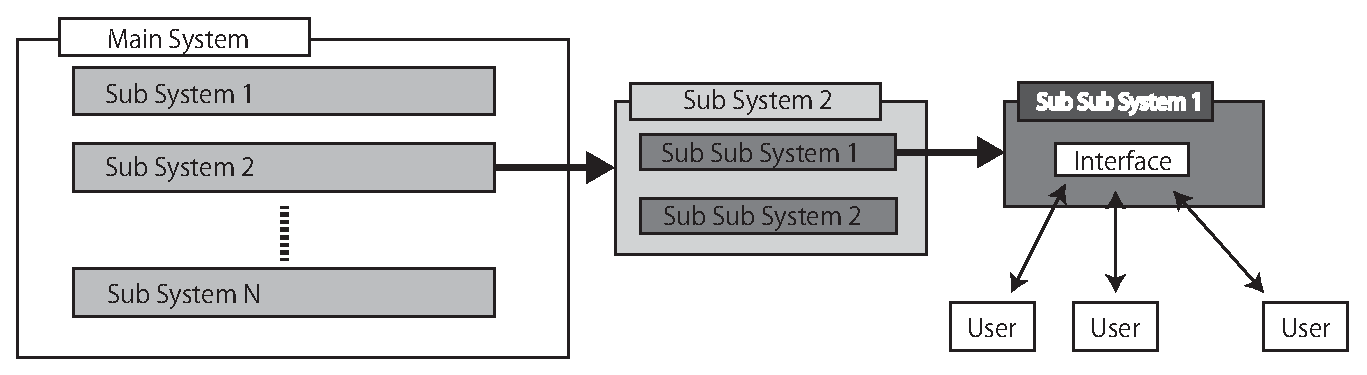
\includegraphics[keepaspectratio, width=150mm]{images/Fig3.eps}
	\caption{Very long sideways figure using two columns.}
	\label{fig3}
\end{figure*}
%%%%%%%%%%%%%%%%%%%%%%%%%%%%%%%%%%

%%%%%%%%%%%%%%%%%%%%%%%%%%%%%%%%%%%%%%%%%%%%%%%%%%%%%%%%%%%%%%%%
%      スタイルファイルについて
%%%%%%%%%%%%%%%%%%%%%%%%%%%%%%%%%%%%%%%%%%%%%%%%%%%%%%%%%%%%%%%%
\section{スタイルファイル{\tt jsms2014v1.sty}について}

材料のフォーマットに合うように、以下の指定を行っています.

\begin{itemize}
\item 冒頭部分でマージン設定(本サンプルの作成環境(Windows7, WinShell)で,Web掲載の「材料学会WordテンプレートVer1.0」とほぼ同じ配置で出力されるように調整している.
環境により微調整が必要となることが多いので紙出力した上で適宜調整して下さい.)

\item 脚注(footnote)の線の指定

\item 章,説のフォントの指定

\item 図,表のキャプションのフォーマットを指定(\verb|[表\ref{table1}]|などで本文中で引用する.)

\item 文献番号が1)という形となるように指定(\verb|[\cite{アイテム名}]|で本文中で引用する.)

\item 章,説の見出しのフォーマット指定

\item 参考文献のタイトルを,文字間隔を空けてセンタリングして出力するように指定

\item 文献のフォントサイズなどを指定

\item その他のスタイル調整等は,本サンプルファイル中で行っている.
\end{itemize}

%%%%%%%%%%%%%%%%%%%%%%%%%%%%%%%%%%%%%%%%%%%%%%%%%%%%%%%%%%%%%%%%
%      サンプルファイルについて
%%%%%%%%%%%%%%%%%%%%%%%%%%%%%%%%%%%%%%%%%%%%%%%%%%%%%%%%%%%%%%%%
\section{{\tt jsms-sample-2014v1-1.tex}について}

本ファイルを適宜書き換えて使用してください.
以下,注意点や使用方法に関する記述です.

\begin{itemize}
\item 著者名とフッター部分の所属先の記述に使用している「*」記号などは,自動には対応していません.
著者名の記述部分と,フッターの記述部分とで,手動で対応を付けてください.

\item 図の挿入と配置は,figure環境を用いることにより図の番号を自動で付番することができます.
ただし,システムが全体の配置を判断した上で最も適した場所(TeXのコンパイラがそう判断するという意味です)に配置してしまいます.
これを,できるだけ記述した箇所のところに配置するために,\verb|[H]|というオプションを付けています.

\item figure環境による図の配置でどうしてもうまくいかない場合は,手動で図を挿入し,図番号やキャプションも手動で書くという方法があります.例えば

\begin{minipage}{0.8\columnwidth}
{\footnotesize
\begin{verbatim}

\begin{center}
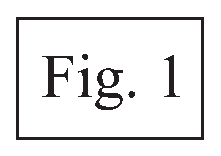
\includegraphics[keepaspectratio, width=50mm]
{images/Fig1.eps}
%
\\
%
\noindent
 {\fontsize{8pt}{0pt}\selectfont
Fig.1 Example
}
\end{center}

\end{verbatim}
}
\end{minipage}

と記述することにより,記述箇所に強制的に図が入ります.ただし,この場合図とキャプションの間に改ページが入ってしまったり,図の途中に改ページ部が来た場合には不釣り合いな空白が入って次のページに図がまわってしまうなどの問題もあります(figure環境を使えば,こういったことは起きません).また,相互参照により図の番号を呼ぶことができなくなります.

\item 参考文献は,\verb|thebibliography| 環境で記述するようにしてあります.この記述スタイルでは,列挙した順番に自動的に1から順番に番号が符されます.

\item 数式は,\verb|equation| 環境を少し変形させた\verb|jsmseq| 環境をマクロで定義してあります.
これは,式番号の右にわずかながら空白を入れるためです.\verb|equation| 環境とほぼ同じように使うことができます.

\item コンパイルを行うと,フォントサイズに関する警告が非常にたくさん出されます.
確認した限りでは,フォントがない場合でも代替フォントでほぼ指定のサイズの文字が出るようになっていると思われます.
新たにフォントをインストールするなどすれば,このあたりの警告は出ないようにできるのではないかと思われます.
\end{itemize}

%%%%%%%%%%%%%%%%%%%%%%%%%%%%%%%%%%%%%%%%%%%%%%%%%%%%%%%%%%%%%
%   参考文献
%%%%%%%%%%%%%%%%%%%%%%%%%%%%%%%%%%%%%%%%%%%%%%%%%%%%%%%%%%%%%
\begin{thebibliography}{99}
%%%%%%%%%%%% 文献リスト %%%%%%%%%%%%%%
\bibitem{Ref01} K. Ohnishi and S. Matsuda, \lq\lq Radiation effects on semiconductor devices: Recent trends of research works\rq\rq, {\textit Journal of the Institute of Electronics and Communication Engineers of Japan}, Vol.85, No.9, pp.662-669 (2002).
%
\bibitem{Ref02} S. Gonda, H. Tsutsumi, Y. Ito, T. Mukai and S. Nagahama, \lq\lq Proton radiation effects in nitride lasers and light emitting diodes\rq\rq, {\textit Physica Status Solidi (a)}, Vol.204, Issue 1, pp.231-235 (2006).
%
\bibitem{Ref03} J. W. Corbett and J. C. Bourgoin, in \lq\lq Point defects in solids\rq\rq , Eds. J. H. Crawford and L. M. Slifkin, p.136 (1975) Plenum Press.
%
\bibitem{Ref04} J. H. Warner, R. J. Walters, S. R. Messenger, G. P. Summers, S. M. Khanna, D. Estan, L. S. Erhardt and A. Houdayer, \lq\lq High-energy proton irradiation effects in GaAs devices\rq\rq, {\textit IEEE Transaction on Nuclear Science}, Vol.51, No.5, pp.2887-2895 (2004).
%
\bibitem{Ref05} S. Gonda, \lq\lq Radiation hardness of InGaAsP semiconductor lasers\rq\rq, {\textit International conference on InP and Related Materials (IPRM)}, WeP29, Versailles France, 2008 May.
%
\bibitem{Ref06} A. Hallen, M. Nawaz, C. Zaring, M. Usman, M. Domeij and M. Ostling, \lq\lq Low-temperature annealing of radiation-induced degradation 4H-SiC bipolar junction transistors\rq\rq, {\textit IEEE Electron Device Letters}, Vol.31, No.7, pp.707-709 (2010).
%
\bibitem{Ref07} S. M. Khanna, D. Estan, L. S. Erhardt, A. Houdayer, C. Carlone, A. I. Nedelcescu, S. R. Messenger, R. J. Walters, G. P. Summers, J. H. Warner and I. Jun, \lq\lq Proton energy dependence of the light output in gallium nitride light-emitting diodes\rq\rq, {\textit IEEE Transaction on Nuclear Science}, Vol.51, No.5, pp.2729-2735 (2004).
%
\bibitem{Ref08} M. Nakano, T. Makino, A. Tsukazaki, K. Ueno, A. Ohtomo, T. Fukumura, H. Yuji, Y. Nishimoto, S. Akasaka, D. Takamizu, K. Nakahara, T. Tanabe, A. Kamisawa and M. Kawasaki, \lq\lq MgxZn1-xO-based schottky photodiode for highly color-selective ultraviolet light detection\rq\rq, {\textit Applied Physics Express}, Vol.1, No.12, pp.121201-1-121201-3 (2008).
%
\bibitem{Ref09} K. Nakahara, S. Akasaka, H. Yuji, K. Tamura, T. Fujii, Y. Nishimoto, D. Takamizu, A. Sasaki, T. Tanabe, H. Takasu, H. Amaike, T. Onuma, S. F. Chichibu, A. Tsukazaki, A. Ohtomo and M. Kawasaki, \lq\lq Nitrogen doped Mg$_{x}$Zn1-$_{x}$O/ZnO single heterostructure ultraviolet light-emitting diodes on ZnO substrates\rq\rq , Applied Physics Letters, Vol.97, No.1, pp.013501-1-013501-3 (2010).
%
\bibitem{Ref10} S. Sasa, T, Hayafuji, M. Kawasaki, K. Koike, M. Yano and M. Inoue, \lq\lq Improved stability of high-performance ZnO/ZnMgO hetero-MISFETs\rq\rq , {\textit IEEE Electron Device Letters}, Vol.28, No.7, pp.543-545 (2007).
%
\bibitem{Ref11} E.g., \lq\lq {\textit Recent development of thin film compound semiconductor photovoltaic cells}\rq\rq , Ed. T. Wada (2007) CMC Press.
%
\bibitem{Ref12} S. O. Kucheyev, P. N. K. Deenapanray, C. Jagadish, J. S. Williams, M. Yano, K. Koike, S. Sasa and M. Inoue, \lq\lq Electrical isolation of ZnO by ion bombardment\rq\rq , Applied Physics Letters, Vol.81, No.18, pp.3350-3352 (2002).
%
\bibitem{Ref13} S. M. Khanna, J. Webb, H. Tang, A. J. Houdayer and C. Carlone, \lq\lq 2 MeV proton radiation damage studies of gallium nitride films through low temperature photoluminescence spectroscopy measurement\rq\rq , {\textit IEEE Transaction on Nuclear Science}, Vol.47, No.6, pp.2322-2328 (2000).
%
\bibitem{Ref14} SRIM simulation, {\tt http://www.srim.org/}
%
%%%%%%%%%%%%%%%%%%%%%%%%%%%%%%%%%%%
\end{thebibliography}

%%%% bibtex未対応(bstファイル未作成) %%%%%
%\bibliography{sample}
%%%%%%%%%%%%%%%%%%%%%%%%%%%%%%%%%%%%

\end{multicols}
}% 本文の9pt指定終了
\end{document}